% ----------------------------------------------------
% Introduction
% ----------------------------------------------------
\documentclass[class=report,11pt,crop=false]{standalone}
% Page geometry
\usepackage[a4paper,margin=20mm,top=25mm,bottom=25mm]{geometry}

% Font choice
\usepackage{lmodern}

% Wrap text around image
\usepackage{wrapfig}

% Checkmarks
\usepackage{tikz}

% For algorithms
\usepackage[]{algorithm}
% Pseudocode packages
\usepackage{algpseudocode}

% Table color
% \usepackage{colortbl}

% Multiple rows
\usepackage{multirow}

% Lorem ipsum
\usepackage{lipsum}

% Use IEEE bibliography style
\bibliographystyle{IEEEtran}

% Line spacing
\usepackage{setspace}
\setstretch{1.20}

% Ensure UTF8 encoding
\usepackage[utf8]{inputenc}

% Language standard (not too important)
\usepackage[english]{babel}

% Skip a line in between paragraphs
\usepackage{parskip}

% For the creation of dummy text
\usepackage{blindtext}

% Math
\usepackage{amsmath}

% Lists
\usepackage{enumitem}

% Header & Footer stuff
\usepackage{fancyhdr}
\pagestyle{fancy}
\fancyhead{}
\fancyhead[R]{\nouppercase{\rightmark}}
\fancyfoot{}
\fancyfoot[C]{\thepage}
\renewcommand{\headrulewidth}{0.0pt}
\renewcommand{\footrulewidth}{0.0pt}
\setlength{\headheight}{13.6pt}

% Epigraphs
\usepackage{epigraph}
\setlength\epigraphrule{0pt}
\setlength{\epigraphwidth}{0.65\textwidth}

% Colour
\usepackage{color}
%\usepackage[usenames,dvipsnames]{xcolor}

% Hyperlinks & References
\usepackage{hyperref}
\definecolor{linkColour}{RGB}{77,71,179}
\hypersetup{
    colorlinks=true,
    linkcolor=linkColour,
    filecolor=linkColour,
    urlcolor=linkColour,
    citecolor=linkColour,
}
\urlstyle{same}

% Automatically correct front-side quotes
\usepackage[autostyle=false, style=ukenglish]{csquotes}
\MakeOuterQuote{"}

% Graphics
\usepackage{graphicx}
\graphicspath{{Images/}{../Images/}}
\usepackage{makecell}
\usepackage{transparent}

% SI units
\usepackage{siunitx}

% Microtype goodness
\usepackage{microtype}

% Listings
\usepackage[T1]{fontenc}
\usepackage{listings}
\usepackage[scaled=0.8]{DejaVuSansMono}

% Custom colours for listings
\definecolor{backgroundColour}{RGB}{250,250,250}
\definecolor{commentColour}{RGB}{73, 175, 102}
\definecolor{identifierColour}{RGB}{196, 19, 66}
\definecolor{stringColour}{RGB}{252, 156, 30}
\definecolor{keywordColour}{RGB}{50, 38, 224}
\definecolor{lineNumbersColour}{RGB}{127,127,127}
\lstset{
  language=Matlab,
  captionpos=b,
  aboveskip=15pt,belowskip=10pt,
  backgroundcolor=\color{backgroundColour},
  basicstyle=\ttfamily,%\footnotesize,        % the size of the fonts that are used for the code
  breakatwhitespace=false,         % sets if automatic breaks should only happen at whitespace
  breaklines=true,                 % sets automatic line breaking
  postbreak=\mbox{\textcolor{red}{$\hookrightarrow$}\space},
  commentstyle=\color{commentColour},    % comment style
  identifierstyle=\color{identifierColour},
  stringstyle=\color{stringColour},
   keywordstyle=\color{keywordColour},       % keyword style
  %escapeinside={\%*}{*)},          % if you want to add LaTeX within your code
  extendedchars=true,              % lets you use non-ASCII characters; for 8-bits encodings only, does not work with UTF-8
  frame=single,	                   % adds a frame around the code
  keepspaces=true,                 % keeps spaces in text, useful for keeping indentation of code (possibly needs columns=flexible)
  morekeywords={*,...},            % if you want to add more keywords to the set
  numbers=left,                    % where to put the line-numbers; possible values are (none, left, right)
  numbersep=5pt,                   % how far the line-numbers are from the code
  numberstyle=\tiny\color{lineNumbersColour}, % the style that is used for the line-numbers
  rulecolor=\color{black},         % if not set, the frame-color may be changed on line-breaks within not-black text (e.g. comments (green here))
  showspaces=false,                % show spaces everywhere adding particular underscores; it overrides 'showstringspaces'
  showstringspaces=false,          % underline spaces within strings only
  showtabs=false,                  % show tabs within strings adding particular underscores
  stepnumber=1,                    % the step between two line-numbers. If it's 1, each line will be numbered
  tabsize=2,	                   % sets default tabsize to 2 spaces
  %title=\lstname                   % show the filename of files included with \lstinputlisting; also try caption instead of title
}

% Caption stuff
\usepackage[hypcap=true, justification=centering]{caption}
\usepackage{subcaption}

% Glossary package
% \usepackage[acronym]{glossaries}
\usepackage{glossaries-extra}
\setabbreviationstyle[acronym]{long-short}

% For Proofs & Theorems
\usepackage{amsthm}

% Maths symbols
\usepackage{amssymb}
\usepackage{mathrsfs}
\usepackage{mathtools}

% For algorithms
%\usepackage[]{algorithm2e}

% Spacing stuff
\setlength{\abovecaptionskip}{5pt plus 3pt minus 2pt}
\setlength{\belowcaptionskip}{5pt plus 3pt minus 2pt}
\setlength{\textfloatsep}{10pt plus 3pt minus 2pt}
\setlength{\intextsep}{15pt plus 3pt minus 2pt}

% For aligning footnotes at bottom of page, instead of hugging text
\usepackage[bottom]{footmisc}

% Add LoF, Bib, etc. to ToC
\usepackage[nottoc]{tocbibind}

% SI
\usepackage{siunitx}

% For removing some whitespace in Chapter headings etc
\usepackage{etoolbox}
\makeatletter
\patchcmd{\@makechapterhead}{\vspace*{50\p@}}{\vspace*{-10pt}}{}{}%
\patchcmd{\@makeschapterhead}{\vspace*{50\p@}}{\vspace*{-10pt}}{}{}%
\makeatother
\makenoidxglossaries

\newacronym{radar}{RADAR}{Radio Detection and Ranging}
\begin{document}
	% ----------------------------------------------------
	\chapter{Methodology \label{ch:meth}}
	%\epigraph{Philosophers have hitherto only interpreted the world in various ways; the point is to change it.}%
	%    {\emph{---Karl Marx}}
	%\vspace{0.5cm}
	% ----------------------------------------------------
	
	%\lipsum[1]
	\section{Methodology Outline}
	
	This chapter details the design process and approach employed in achieving the aim of the project which is to  digitize and modernize the HP141T display by replacing the \acrshort{crt} monitor with a \acrshort{lcd} touchscreen display that offers different functions and modes of operation. Design decision are also documented here, showing the considerations that were made based on the operation and outputs of the HP141T spectrum analyzer and ensuring that the newly integrated display is compatible with the device's hardware. For example, the design required selection of the digital hardware for processing the analog voltage signals from the \acrshort{sa}. The selection of the digital processor made from single-board computers such as the Raspberry Pi 4 Model B, microcontrollers like the STM32F4 boards, \acrshort{fpga} such as the Artix-7 from Xilinix, or a heterogeneous digital processor which consists of a combination of these options. 
	
	Other considerations were made regarding the electronic circuits for converting the auxiliary output voltages from the HP141T to the appropriate voltage level for the operation of \acrshort{adc}. This chapter describes how together, the \acrshort{adc} and digital processor form a crucial part of the system. Additionally, the chapter details the software development kit (\acrshort{sdk}) and associated coding language that was used. The selection of the development framework depended on the choice of processor and digital processing algorithms that were required to fulfil the project requirements. For example, assuming that a \acrshort{fpga} is the chosen digital processor, the  \acrshort{sdk} would include tools such as the AMD Vivado and electronic design automation (\acrshort{eda}) software and the choice of coding language between Verilog, VHDL, and SystemVerilog would depend on how comfortable the developer is in representing digital processing algorithms, such the \acrshort{dft}, using the chosen language. 
	
	Overall, this chapter documents an overview of the design methodology and different phases in the design process. The design process followed a variation of V-Model in which a series of iterative phases was implemented with a process checking mechanism. The chapter begins by highlighting the design stages and modularization of the system. Thereafter, the chapter includes an assessment of the project requirements detailed in introductory section. Finally, the chapter describes the use of findings from the review of requirements in informing the design decisions and specifications.  
	
	\section{Phases in the Design Process}
	
	The design process was decomposed into four iterative stages as illustrated in Figure \ref{fig:design-stages-diagram} below. The first stage documented the digitization requirements and listed examples of modern \acrshort{sa}s in order to define the requirements for modernization. As shown in the methodology overview diagram, the first stage also included thorough investigation into methods that have been implemented in literature for upgrading the functions and performance of \acrshort{sa}s. A theoretical framework for relevant information about signal processing was also formulated based on the literature to ensure that the display modes and functions were consistent with the mathematically derived expected outputs in the system. 
	
	\begin{figure}[!ht]
		\centering
		\label{fig:design-stages-diagram}
		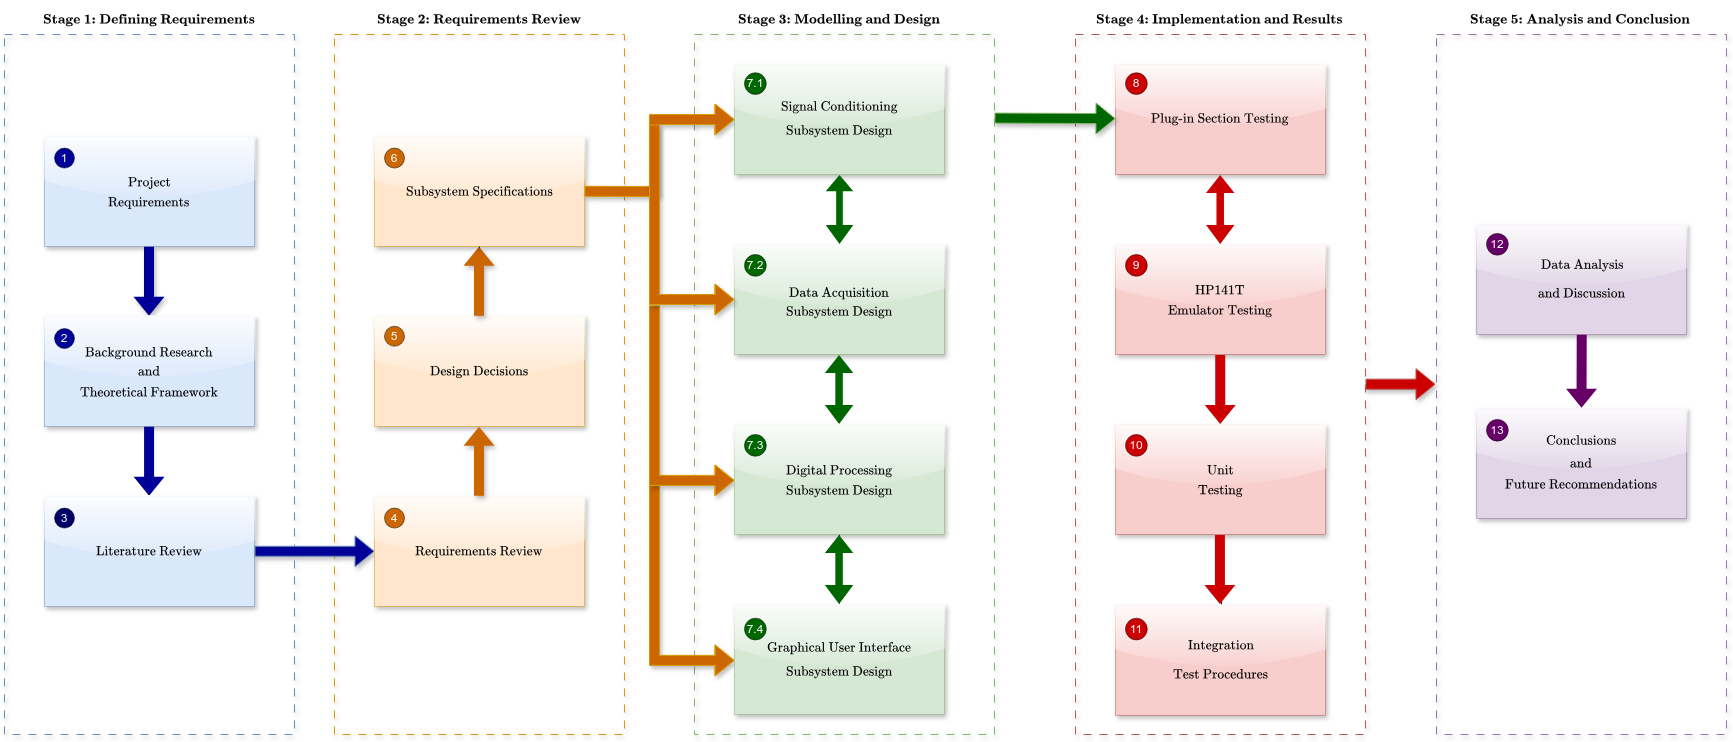
\includegraphics[width=1.0\linewidth]{Figures/Methodology/design-stages-diagram.png}
		\caption{Methodology overview showing different stages in the iterative design process that was applied as a variation of the V-Model.}
	\end{figure}
	
	The second stage in the design process involved a review of the user requirements specifications detailed in chapter \ref{ch:intro}. The aim of this step in the methodology was to clarify the desired functions of the upgraded spectrum analyzer and to inform the design decisions with respect to the digital hardware and software development for digital signal processing. Additionally, the requirements review was employed in modularizing the design into four subsystems including, the Analog-to-Digital Conversion, Digital Processing, Screen and User Interface subsystems. 
		
	Stage 3 of the design process dealt with the design specifications of each of these subsystems by further decomposing each module into smaller hardware and software components. Each function is tested against a requirement in Stage 4 where each design specification was verified and the operation of the integrated system was tested to ensure that the interfaces between the subsystems was configured correctly. 
	
	In general, implementation of the design process adhered to the following design steps detailed in the project brief and are associated with the user requirement specifications:
	
	\begin{enumerate}
		\item 
		Surveying the HP141T display and other outputs.
		\item 
		Surveying single-board computers and touchscreen options.
		\item 
		Phase One: establish a basic XYZ replica or HP141T emulator.
		\item 
		Phase Two: implement averaging and peak hold options.
		\item 
		Phase Three: annotate display axes.
		\item 
		Phase Four: determine the appropriate instrument settings. 
		\item 
		Phase Five: design new annotations for display taking instrument or operator manual inputs into account.
		\item 
		Phase Six: include more tutorial and operational instructions using.
	\end{enumerate}
	
	In finalizing the design process of the upgraded \acrshort{sa}, results from acceptance tests were assimilated and a conclusion was drawn. Then, based on the outcomes of the project, future recommendations were made for future iterations of the upgrade \acrshort{sa} system. Overall, the stages of the methodology included:
	
	\begin{itemize}
		\item 
		Stage 1: Defining Requirements
		\item 
		Stage 2: Requirements Review and System Overview
		\item 
		Stage 3: Modelling and Design
		\item 
		Stage 4: Implementation and Results
		\item 
		Stage 5: Analysis and Conclusion 
	\end{itemize}

	The first four stages of the design process were performed iteratively as a variation of the V-Model in which risk analysis was performed at each step, similar to the Spiral Model for design processes. Each iteration aimed at producing a new version of the upgraded HP141T display and a single conclusion was made when a satisfactory prototype was established.

	\section{Requirements Review}
	
	This section aims to clarify the scope of the project and produce a technical formalization of the user requirements specifications. The section begins by giving context to the term modernization by investigating the properties of modern \acrshort{sa}s. Then, the section breaks down the user requirements into categories relating data acquisition, processing and display. Finally, the section concludes with a review of the requirement for developing a HP141T emulator. 
		
	\subsection{Comparing the HP141T System to Modern Spectrum Analyzers}
	
	The first user requirement deals with the modernization of the HP141T system. The aim of this section is to review this requirement and to give clarification on the context of the use of "modernization" in this project. To achieve this objective, the section begins with a description of the HP141T system and the functions that differ from "modern" spectrum analyzers, such as the range of hand-held \acrshort{sa}s by FieldFox, and the N9000B CXA \acrshort{sa} manufactured by Keysight\textregistered. The section concludes with a summary table comparing the features of the HP141T system and modern spectrum analyzers. 
	
	The HP141T system is equipped with three plug-ins, namely the 8555A \acrshort{rf} section which operates in the microwave region of the electromagnetic spectrum, the 8552B \acrshort{if} section and the Model 141T display which includes the \acrshort{crt} monitor. The three plug-ins operate in unison to electronically scan signals in the time-domain and provide a visual representation of the input signal's amplitude in the frequency domain on the \acrshort{crt} monitor \cite{HP8555A}. Amplitude can be represented on a logarithmic ($\si{\decibel\meter}$) or linear scale ($\si{\milli\volt}$). 
	
	The 8555A and 8552B plug-ins apply principles of heterodyning spectroscopy, allows high frequency input signals with frequencies in the K-band of the microwave portion of the electromagnetic spectrum (i.e. $\SI{18}{\mega\hertz}$) \cite{harris2003}. As noted from literature in the previous chapter, spectrum analyzers which rely on the \acrshort{fft} by sampling the continuous input signal and performing the Fourier transform on $N$ total samples typically deal with signals that have lower frequencies. This is because \acrshort{sa}s that employ the super-heterodyne principle like the HP141T determine the spectrum directly by analysis in the frequency domain and not from the time-dependent characteristics of the input signal. This is achieved by using a super-heterodyne receiver comprised of a mixer and tunable local oscillator (\acrshort{lo}) which convert the input signal to an intermediate frequency as illustrated in figure \ref{fig:heterodyne-rauscher} \cite{rauscher2007}. 
	
	\begin{figure}[!ht]
		\centering
		\label{fig:heterodyne-rauscher}
		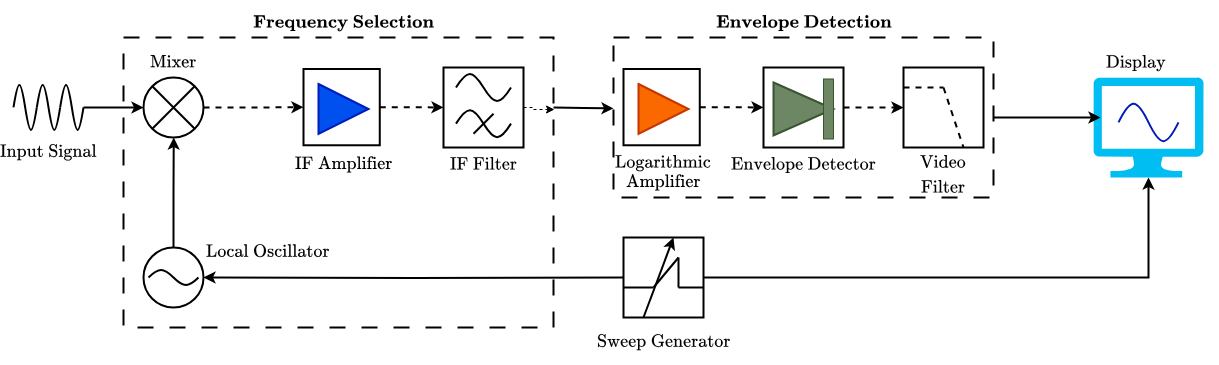
\includegraphics[width=1.0\linewidth]{Figures/Methodology/heterodyne-rauscher.png}
		\caption{Heterodyne Spectrum Analyzer Block Diagram.}
	\end{figure}
	
	As noted in the literature review, most modern \acrshort{sa}s are real-time spectrum analyzers \acrshort{rtsa} which are a special case of vector spectrum analyzers (\acrshort{vsa}) that use the super-heterodyne principle but digitize the input signal at the intermediate frequency, as shown in Figure \ref{fig:vector-analyzer-rover}, using a bandpass filter which can behave like a pre-select filter to limit distortions that arise from the mixer and shows the result in real-time. The advantage of digitizing the output of the \acrshort{if} section is that it enables large a input range of up to $\SI{50}{\mega\hertz}$ which can be analyzed in the time and frequency domain using digital signal processing techniques \cite{rovers2006}. Much like \acrshort{fft} analyzers, vector analyzers are limited by the minimum and maximum sampling rate at which the \acrshort{adc} can operate. Additionally, exceedingly high sampling rates can lead to aliasing which causes frequencies outside of the bandwidth to fold into the frequency band \cite{rovers2006}. 	

	\begin{figure}[!ht]
		\centering
		\label{fig:vector-analyzer-rover}
		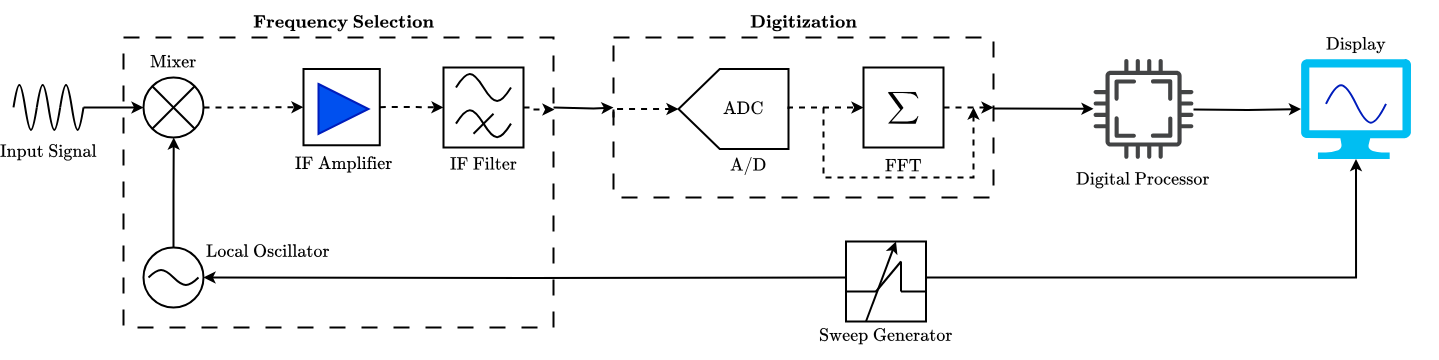
\includegraphics[width=1.0\linewidth]{Figures/Methodology/real-time-analyzer-rover.png}
		\caption{Vector analyzer block diagram showing digitization of the \acrshort{if} frequency.}
	\end{figure}

	Examples of modern real-time analyzers include:
	
	\begin{itemize}
		\item 
		Tektronix RSA2208A which can scan input signals with frequencies of up to $\SI{8}{\giga\hertz}$.
		\item 
		Rohde \& Schwarz FSP13 which operates within a $\SI{9}{\giga\hertz}$ to $\SI{30}{\giga\hertz}$ \acrshort{rbw}.
		\item
		Agilent E4445A which offer frequency analysis up to $\SI{13.2}{\giga\hertz}$.
		\item 
		FieldFox RTSA which covers $\SI{5}{\kilo\hertz}$ up to $\SI{50}{\giga\hertz}$.
	\end{itemize}

	In modern \acrshort{rtsa}s, \acrshort{if} analog output is transferred to the \acrshort{adc} through an anti-aliasing filter before being stored in memory \cite{tektronixRSA2208A}. This is in contrast to older heterodyne \acrshort{sa}s such as the HP141T which takes the \acrshort{if} output through a video filter is essentially an averaging low-pass filter which smooths the \acrshort{if} output and reduces the effects of internal noise before the signal is channelled to the display \cite{rauscher2007}. HP141T video filters may select $\SI{10}{\hertz}$, $\SI{100}{\hertz}$, $\SI{10}{\kilo\hertz}$ or OFF section of the low-pass filter for the detected video. 
	
	In the HP141T, the output of the video filter is transmitted to the vertical deflection of the \acrshort{crt} display \cite{HPsiganalyzers}. For the horizontal deflection of the electron beam in the \acrshort{crt} display, a sawtooth signal from the sweep generator governs the horizontal scaling of the output frequency as electrons impinge on the phosphorescent screen. Modern \acrshort{sa}s retrieve data from memory through high speed data lines to display information about the digital signal from the \acrshort{adc}. Digital display technologies include:
	
	\begin{itemize}
		\item 
		\acrshort{lcd} - most commonly used digital display which represents signal data with a sharp image and has low power consumption
		\item 
		\acrshort{oled} - typically used in high performance \acrshort{sa}s for displaying color coded spectrograms
		\item 
		\acrshort{tft} - offer good visual quality and response time for sharper imagery when analyzing high frequency signals.
	\end{itemize}

	Displays in modern \acrshort{sa} architectures offer more options for displaying frequency domain data. This is enabled by the processor, which is typically hosted on microcontroller board with high clock speed for performing digital signal processing algorithms. For example, \acrshort{rtsa}s display the spectrogram as a color coded function of the amplitude of the signal \cite{al2013}. In addition, digital displays generally consume less physical space compared to \acrshort{crt} displays with the same screen dimensions. This has allowed spectrum analyzers to become smaller as they entire system can fit into smaller packaging. For example, the FieldFox is an hand-held \acrshort{rtsa} which despite its size, offers improved performance over the HP141T.
	
	The comparison table in \ref{tab:comparing-old-to-modern} below summarizes the differences between the HP141T analyzer (equipped with the 8555A and 8552B plug-ins) and modern \acrshort{rtsa}s.
	
	 \begin{table}[ht!]
	 	\centering
	 	\begin{tabular}{|m{8em}|m{15em}|m{15em}|}
	 		\hline
	 		\cellcolor{cyan!25}\textbf{Feature}	& \cellcolor{cyan!25}\textbf{HP141T}	& \cellcolor{cyan!25}\textbf{Real-Time Spectrum Analyzer}\\
	 		\hline
	 		Operation &	Heterodyne	&	\acrshort{fft}-based real-time processing\\
	 		\hline
	 		Frequency Range &	$\SI{10}{\giga\hertz}$	- $\SI{40}{\giga\hertz}$	&	DC to $\SI{54}{\giga\hertz}$\\
	 		\hline
	 		Scan Speed &	$\SI{0.1}{\milli\second}/\text{div}$ - $\SI{10}{\second}/\text{div}$	&		Real-time GHz bandwidth capture with no losses\\
	 		\hline
	 		Dynamic Range	&	High but limited by analog filters	& Very high due to digital signal processing\\
	 		\hline
	 		Resolution Bandwidth	&	Adjustable limited by analog filters	&	As low as $\SI{1}{\hertz}$\\
	 		\hline
	 		Real-time Capture	&	No. Displays active signals and struggles with pulsed signals &	Yes. Captures transient and pulsed signals with ease\\
	 		\hline
	 		Signal Processing	&	Analog signal processing with IF filters and logarithmic amplifiers	& Digital signal processing from \acrshort{adc}-sampled signal\\
	 		\hline
	 		FFT Capability	&	- &	Built-in FFT \\
	 		\hline
	 		Display Type	&	\acrshort{crt}	&	\acrshort{lcd}/\acrshort{oled}/\acrshort{tft}\\
	 		\hline
	 		Trace Storage	&	No memory. &	Digital data storage\\
	 		\hline
	 		Connectivity	&	None &	\acrshort{usb}, Wi-Fi, Bluetooth, \acrshort{ble}\\
	 		\hline
	 		Size \& Portability	&	Large and mountable on a rack &	Compact and portable\\
	 		\hline
	 		Settings \& Configuration	&	Manual tuning and calibration	&	Automated measurements, presets, user-friendly\\
	 		\hline
	 	\end{tabular}
 		\caption{Comparing the features of the HP141T system to the modern \acrshort{rtsa}s.}
 		\label{tab:comparing-old-to-modern}
	 \end{table}
	
	Table \ref{tab:comparing-old-to-modern} shows that \acrshort{rtsa}s also have connectivity abilities. For example, data can be transferred serially from on-board memory to an external device through the \acrshort{usb} transfer protocol or through the \acrshort{ble} transfer protocol. 
	
	Features shown in the comparison formulated the modernization criteria to give context to the user requirement specification. Following sections expand on the features which can provide the functionality for associated requirements. 
	
	\subsection{Data Acquisition in Digitizing the HP141T}
	
	As seen in the previous section, a primary criteria for modernizing HP141T is the translation of continuous analog input signals from the time domain to a digital signal that can be assessed using a digital processor such as a single-board computer, \acrshort{fpga}, or microcontroller. Selecting the point at which the conversion occurs in the pipeline of the HP141T super-heterodyne system plays a crucial role in the performance of the modernized system. The following project aimed to fulfil the signal conversion criteria by sampling the input signal at the intermediate frequency in a similar manner to the technique implemented by a modern \acrshort{rtsa} and vector analyzers. In addition, user requirement UR01 states that the system needs to sample 801 points which is a standard for modern signal analyzers.
	
	The following section reviews the user requirements to inform decisions about the data acquisition subsystem of the digitized HP141T subsystem. One of the most crucial parts in the design of the data acquisition subsystem is the selection of the \acrshort{adc} which samples signals and transmits them to the digital processor to store or manipulate signals in real-time. The section describes the limitations of this central part of the system and proposes solutions that can be implemented to fulfil the user requirements.
			
	\subsubsection{\acrshort{adc} Constraints}
	
	Table \ref{tab:adc-constraints} shows constraints that influence the selection of the \acrshort{adc} and a solution for circumventing the limitation. For example, the operating voltage range of the \acrshort{adc} is a constraint which can be circumvented by including a signal conditioning circuit.
	
	\begin{table}[!ht]
		\centering
		\begin{tabular}{|m{8em}|m{15em}|m{15em}|}
			\hline
			\cellcolor{cyan!25}\textbf{Constraint}	& \cellcolor{cyan!25}\textbf{Problem}	& \cellcolor{cyan!25}\textbf{Solution}\\
			\hline
			Operating Voltage	& Limited input voltage range of $\SI{0}{\volt}$ to $\SI{3.3}{\volt}$ or $\SI{5.0}{\volt}$. The HP141T produces incompatible auxiliary output voltages	& Signal conditioning circuit for scaling and shifting signals for compatibility with \acrshort{adc} operating voltages\\
			\hline
			Sample Rate			& Required minimum of 801 points & Select an \acrshort{adc} with a high sampling rate (at 1 \acrshort{msps}) \\
			\hline
			Resolution			& Higher resolution is required for finer amplitude accuracy	& Use an \acrshort{adc} with a minimum resolution of 16-bits\\
			\hline
			Number of Channels	& The HP141T has 3 auxiliary outputs that are related to the frequency vs amplitude plot 	& Use an \acrshort{adc} with at least 3 channels\\
			\hline
			Latency				& High latency can introduce delays in rendering signal data in real-time	& Choose an \acrshort{adc} with \acrshort{spi} for low latency\\
			\hline
			\acrshort{snr}	& \acrshort{adc} with a low \acrshort{snr} are more susceptible to noise and fluctuations in the amplitude 	&	Use an \acrshort{adc} with a high \acrshort{snr}\\
			\hline
		\end{tabular}
		\label{tab:adc-constraints}
		\caption{\acrshort{adc} selection constraints and solutions.}
	\end{table}

	\subsubsection{Conditioning HP141T Output Voltages to Match the \acrshort{adc} Operating Voltages}
	
	To satisfy the modernization requirement, an \acrshort{adc} with at least three channels is required to sample the three auxiliary analog output signals from the HP141T system that are shown in Table \ref{tab:hp141t-output-voltages} below.
	
	\begin{table}[!ht]
		\centering
		\begin{tabular}{|m{5em}|m{8em}|m{25em}|}
			\hline
			\cellcolor{cyan!25}\textbf{Name} & \cellcolor{cyan!25}\textbf{Range} & \cellcolor{cyan!25}\textbf{Description}\\
			\hline
			 Pen-Lift	&$\SI{0}{\volt}$ to $\SI{14}{\volt}$ & Triggers the \acrshort{crt} display. The pen-lift output is $\SI{0}{\volt}$ during scanning\\
			\hline
			Vertical Output	& $\SI{0}{\volt}$ to -$\SI{0.8}{\volt}$	& Detected video output proportional to the vertical deflection on the \acrshort{crt}, corresponding to the amplitude of the signal in the frequency domain. Voltage range is scaled for full vertical deflection of the electron beam in 8 divisions of the \acrshort{crt} display \\
			\hline
			 Horizontal Output	& -$\SI{5}{\volt}$ to $\SI{5}{\volt}$ & Sawtooth signal for representing scaling frequency across 10 divisions of the horizontal deflection on the \acrshort{crt} display. The HP141T uses this output to control the trace of the spectrum across the screen. \\
			\hline
		\end{tabular}
		\label{tab:hp141t-output-voltages}
		\caption{Auxiliary voltages of the HP141T that must be sampled to digitize the system.}
	\end{table}

	Since the operating voltage of most \acrshort{adc}s is in the range between $\SI{0}{\volt}$ and $\SI{3.3}{\volt}$ or $\pm\SI{5}{\volt}$, the auxiliary outputs listed in table \ref{tab:hp141t-output-voltages} need to be scaled and shift to be within the operating voltage range. To scale the signal, an op-amp with appropriate gain $A$ can be used between the auxiliary outputs of the HP141T and the input channels of the \acrshort{adc}. To shift the output voltages, a logic level-shifter can be used to translate the signals to be within the operating voltage domain. 

	\subsubsection{Sampling Limitations in the Data Acquisition and Data Processing Subsystems}
		
	Among the constraints in the selection of the \acrshort{adc} is the requirement of the data acquisition subsystem to sample 801 points. Given that the 8552B has 16 internal scan rates from $\SI{0.1}{\milli\second}/\text{div}$ to $\SI{10}{\second}/\text{div}$ in a 1, 2, 5 sequence and given that the data acquisition subsystem needs to store 801 points per scan, the fastest scan rate, corresponding to $\SI{0.1}{\milli\second}/\text{div}$, can be achieved using an \acrshort{adc} with a sampling rate of 
	\begin{align}
		\frac{801\text{samples}}{\SI{0.1}{\milli\second}}	& = 8.01~\textbf{\acrshort{msps}}\nonumber
	\end{align}
	Similarly, for the slowest scan rate corresponding to $\SI{10}{\second}/\text{div}$, the required minimum sampling rate of the \acrshort{adc} is 80.1 \acrshort{sps}.
	
	In addition to the sample rate of the \acrshort{adc}, the design must take several factors into account regarding the integration of the \acrshort{adc} with a digital processor such as a \acrshort{sbc}, \acrshort{mcu}, or \acrshort{fpga}. Table \ref{tab:digital-processor-considerations} shows the considerations that need to be made in selecting a digital processor that is compatible with the operation of the \acrshort{adc} and high sampling rate.
	
	\begin{table}[!ht]
		\centering
		\begin{tabular}{|m{5em}|m{15em}|m{20em}|}
			\hline
			\cellcolor{cyan!25}\textbf{Digital Processor Type}	& \cellcolor{cyan!25}\textbf{Consideration}	&	\cellcolor{cyan!25}\textbf{Feature}\\
			\hline
			\multirow{3}*{\acrshort{mcu}}	& Communication Interface &	Supports $\text{I}^2\text{C}$ and \acrshort{spi} \\
			\cline{2-3}
			& Data Transfer Rate & Up to hundreds of $\si{\mega\hertz}$\\
			\cline{2-3}
			& Synchronization and Timing &	Can use interrupts and \acrshort{fifo} buffers \\
			\hline
			\multirow{3}*{\acrshort{sbc}}	& Communication interface	& Supports $\text{I}^2\text{C}$ and \acrshort{spi}	\\
			\cline{2-3}
			& Data Transfer Rate & Suited for low sampling rates\\
			\cline{2-3}
			& Synchronization and Timing & Requires buffering and introduces operating system relating delays\\ 
			\hline
			\multirow{3}*{\acrshort{fpga}}	&	Communication Interface & Supports \acrshort{spi} and high-speed parallel interfaces\\
			\cline{2-3}
			& Data Transfer Rate & Can handle sampling rates at hundreds of $\si{\mega\hertz}$ to $\si{\giga\hertz}$ speeds.\\
			\cline{2-3}
			& Synchronization and Timing &	Uses parallel data pipelines suitable for high-speed sampling rates for real-time spectral analysis applications.\\
			\hline
		\end{tabular}
		\caption{Digital processor selection based on \acrshort{adc} interface considerations.}
		\label{tab:digital-processor-considerations}
	\end{table}
		 
	Table \ref{tab:digital-processor-considerations} indicates that to fulfil the requirement for sampling 801 points per scan, the design that can deliver the highest performance in real-time data acquisition should include an \acrshort{adc} which can perform 8.01 \acrshort{msps} and a \acrshort{fpga} with multiple pipelines for storing and processing rapidly sampled data in parallel. Alternatively, a heterogeneous digital processor can be implemented using a suitable combination of the available options listed in the table. For example, a Xilinx Artix-7 \acrshort{fpga} can be used for high-speed data acquisition while a Raspberry Pi \acrshort{sbc} is used to process and display data. \acrshort{mcu}s can also be daisy-chained to perform different tasks in the data acquisition subsystem. 
	
	\subsubsection{Further Design Considerations in Digital Processor Selection}
	
	While \acrshort{fpga}s offer superior speeds in data acquisition and processing, one of the shortcomings of selecting it as the primary digital processor is that the overall development time is typically longer than the design time for \acrshort{mcu}s and \acrshort{sbc}s. This is because \acrshort{fpga} development has a structured design flow which includes details of the register-transfer level (\acrshort{rtl}) using a hardware description language (\acrshort{hdl}), validation, synthesis and implementation. Although tools like AMD Vivado exist to significantly reduce \acrshort{fpga} development times, the other available options offer significantly shorter development times. 
	
	Table \ref{tab:digital-processor-comparison} gives a comparison between the available digital processor options to highlight the most suitable option for fulfilling the requirements of this project. 
	
	\begin{table}[ht!]
		\centering
		\label{tab:digital-processor-comparison}
		\begin{tabular}{|m{8em}|m{10em}|m{10em}|m{10em}|}
			\hline
			\cellcolor{cyan!25}\textbf{Design Aspect}	&	\cellcolor{cyan!25}\textbf{\acrshort{mcu}}	&	\cellcolor{cyan!25}\textbf{\acrshort{sbc}}	&	\cellcolor{cyan!25}\textbf{\acrshort{fpga}}\\
			\hline
			Development Time	&	Short	&	Moderate	& 	Long\\
			\hline
			Processing Speed	& 	Medium	&	Moderate to High	& 	High\\
			\hline
			Programming Language	& C/C++ &	Python or C/C++	 & VHDL or Verilog\\
			\hline
			On-board Memory and \acrshort{ram}	& Very Low & High	& Low\\
			\hline
			Power consumption	& Low	& High	& Moderate to High\\
			\hline
			Scalability		& High	& Moderate	& High \\
			\hline
			Cost	& Low	& Moderate to High	& High\\
			\hline	
		\end{tabular}
		\caption{A structure comparison of the available digital processor options.}
	\end{table}

	The different benefits of choosing a certain digital processor can be deduced from Table \ref{tab:digital-processor-considerations} and \ref{tab:digital-processor-comparison}. Other considerations need to made regarding the memory capacity of the chosen processor, however, the primary objective is to satisfy UR06 which requires the data acquisition subsystem to be capable of storing and recalling traces. Due to the high sampling rate, the device must have a sufficient large memory capacity for storing signal frequency and amplitude related information at high-speeds. Specifically, given that a minimum sampling rate of 8.01 \acrshort{msps} is required and supposing that the resolution of the \acrshort{adc} is 16-bit, the device must be able to store
	\begin{align}
		8.01 \text{MSPS} \times \SI{16}{\bit} & = \SI{128160000}{\bit\per\second}\nonumber
	\end{align}
	In other words, the device must be able to store $\SI{16.02}{\mega\byte\per\second}$, which equates to approximately $\SI{1}{\giga\byte}$ per minutes. Thus, the selected digital processor must include efficient memory management algorithms to ensure that data is not lost or corrupted. The table indicates that the \acrshort{mcu} has the most limited capability with respect to memory. This is because \acrshort{mcu}s typically have few KB to MB of \acrshort{ram} and require external memory. Similarly, \acrshort{fpga}s offer limited memory capabilities since they typically use a small embedded \acrshort{ram} and require external memory for large data buffers. 
	
	In summary, the \acrshort{mcu} is most suitable for its low cost, low power consumption, good real-time capabilities and short development time. However, the \acrshort{mcu} is only suitable for moderate-speed sampling, which is not ideal for the high sampling rates that are needed to fulfil the requirements. While \acrshort{sbc}s offer intermediate performs and features that combine the moderate capabilities of \acrshort{mcu}s and \acrshort{fpga}s, their primary shortcoming is poor real-time capabilities due to \acrshort{os} delays and overall low latency. Finally, the best option for this application is the \acrshort{fpga} due to its ability to perform real-time high-speed data processing and \acrshort{adc} synchronization, however, the biggest shortcomings are the development time and high cost. 
	
	\subsection{Design Considerations in Satisfying Display Requirements}
	
	The choice of display depends on the selected processor type. The display hardware must satisfy multiple user requirements including UR03, UR07 and UR09 which are related to resolution, functionality and power. Further considerations have to be made for the display to satisfy requirements relating to the user interface (\acrshort{ui}). The following section breaks down these requirements separately to evaluate the design choices that need to be made in modernizing the HP141T display.
	
	\subsubsection{Display Hardware Considerations for a \acrshort{mcu}-Based System}
	
	Table \ref{tab:mcu-display-options} assimilates the design considerations for a \acrshort{mcu}-based system. Overall, the design needs to consider factors such as clock and I/O speed, memory, power consumption and the display interface.
	
	\begin{table}[ht!]
		\centering
		\begin{tabular}{|m{5em}|m{10em}|m{24em}|}
			\hline
			\cellcolor{cyan!25}\textbf{Key Consideration}	&	\cellcolor{cyan!25}\textbf{Aspects}	& \cellcolor{cyan!25}\textbf{Description}\\
			\hline
			\multirow{3}{*}{Processor}	& Clock Speed	& Clock speed of at least $\SI{100}{\mega\hertz}$ for rendering 801 points per scan to the display\\
			\cline{2-3}
			&	Architecture &	A 32-bit ARM Cortex-M series \acrshort{mcu} is preferred for good balance between power efficiency and speed\\
			\cline{2-3}
			&	I/O Speed & \acrshort{adc} waveform samples need to be rendered at high speeds. \acrshort{spi} is recommended for improving latency\\
			\hline
			\multirow{2}{*}{Memory}	& 	\acrshort{ram}	& At least $\SI{128}{\kilo\byte}$ of \acrshort{ram} required for real-time display rendering\\
			\cline{2-3}
			&	Flash Memory	&	Required for storing firmware and display configurations which need to be loaded during power-up.\\
			\hline
			\multirow{2}{*}{Interface}	&	Compatibility	& Should support the same communication interfaces as the display screen.\\
			\cline{2-3}
			&	Resources &	Modern displays include internal frame buffers which can reduce the effect of memory and data transfer bottlenecks.\\
			\hline
			\multirow{2}{*}{Power}	&	Compatibility & System must be powered by a single wall wart power supply.\\
			\cline{2-3}
			&	Efficiency	&	Low-power and standby modes can reduce energy consumption when the display is idle.\\
			\hline
		\end{tabular}
		\caption{Key considerations for the display subsystem for a \acrshort{mcu}-based system.}
		\label{tab:mcu-display-options}
	\end{table}
	
	\subsubsection{Display Hardware Considerations for a \acrshort{sbc}-Based System}
	
	If the chosen digital processor is a single-board computer such as the Raspberry Pi 4B, similar considerations need to be made regarding its compatibility of the display unit. Differences arise from the hardware capabilities that the \acrshort{sbc} offers. Table \ref{tab:sbc-display-options} summarizes the design considerations that need to be made for the interface between \acrshort{sbc} and the display unit.
	
	\begin{table}[ht!]
		\centering
		\begin{tabular}{|m{5em}|m{10em}|m{24em}|}
			\hline
			\cellcolor{cyan!25}\textbf{Key Consideration}	&	\cellcolor{cyan!25}\textbf{Aspects}	& \cellcolor{cyan!25}\textbf{Description}\\
			\hline
			\multirow{2}{*}{Resolution} 
			& 1080p at 60Hz & Recommended for smooth spectrum rendering; higher resolutions. \\
			\cline{2-3}
			& HDMI 2.0 & A high-speed \acrshort{hdmi} 2.0-compatible display is required for the best display quality. \\
			\hline
			
			\multirow{3}{*}{\acrshort{hdmi}} 
			& \acrshort{hdmi} Version Support & Older monitors may only support HDMI 1.2, which could limit resolution and refresh rates \\
			\cline{2-3}
			& Data Handling & Improper extended display identification data detection may require manual configuration \\
			\cline{2-3}
			& Adapter	& Micro-\acrshort{hdmi} to \acrshort{hdmi} adapters are required. Faulty adapters may introduce noise\\
			\hline
			
			\multirow{3}{*}{Touch} 
			& Touch Display & Dedicated \acrshort{sbc} touchscreens can be used \\
			\cline{2-3}
			& \acrshort{dsi} & Raspberry Pi touchscreen connect via the \acrshort{dsi} (Display Serial Interface) without required \acrshort{hdmi}\\
			\cline{2-3}
			& Power & Dedicated screen can be powered by the \acrshort{sbc}\\
			\hline
			
			\multirow{2}{*}{Monitor} 
			& Compatibility & Selected display must support the required resolution and refresh rate for clear visualization of digitized spectra. \\
			\cline{2-3}
			& Over-scanning & Display adjustments may be required for screens that crop spectrum visualizations. \\
			\hline
						
			\multirow{2}{*}{Software} 
			& OS Support & Dedicated \acrshort{os} recommended for compatibility with built-in display drivers and utilities. \\
			\cline{2-3}
			& Settings & Used to adjust display resolution, rotation, and other settings for the most suitable spectrum visualization. \\
			\hline
		\end{tabular}
		\caption{Display considerations for screen integration with a \acrshort{sbc}-based system.}
		\label{tab:sbc-display-options}
	\end{table}
	
	\subsubsection{Display Hardware Considerations for a \acrshort{fpga}-Based System}
	
	Although \acrshort{fpga}s offer the best performance with respect to sampling rates and data processing speeds, they are not as suitable for processing display data compared to \acrshort{sbc}s. However, the real-time capabilities of the \acrshort{fpga}-based system can provide a seamless user experience by rendering spectrum displays at a high frame rate. Table \ref{tab:fpga-display-options} lists the design considerations for the display of a \acrshort{fpga}-based system.
	
	\begin{table}[ht!]
		\centering
		\begin{tabular}{|m{8em}|m{10em}|m{22em}|}
			\hline
			\cellcolor{cyan!25}\textbf{Key Consideration} & \cellcolor{cyan!25}\textbf{Aspects} & \cellcolor{cyan!25}\textbf{Description} \\
			\hline
			\multirow{3}{*}{Video Output} 
			& \acrshort{hdmi} Support & Different FPGAs feature built-in \acrshort{hdmi}, \acrshort{dvi} transmitters or external serializer chips. The chosen FPGA must support high-speed video output \\
			\cline{2-3}
			& Parallel & For parallel \acrshort{rgb} inputs, the FPGA must generate compatible timing signals for proper synchronization \\
			\cline{2-3}
			& Buffering & Additional external memory may be required for storing video frames before display \\
			\hline
			
			\multirow{2}{*}{Synchronization} 
			& Pixel Clock & Display’s resolution and refresh rate requirements must be compatible with a stable \acrshort{fpga} pixel clock \\
			\cline{2-3}
			& Fabric Speed & Spectrum updates can be rendered rapidly using the high-speed fabric which ensure low-latency \\
			\hline
			
			\multirow{3}{*}{Interface} 
			& Protocols & The display must be able to interface with the available hardware on the \acrshort{fpga} \\
			\cline{2-3}
			& Controller & Display must be compatible with \acrshort{fpga} IP cores for developing display functionality more easily\\
			\cline{2-3}
			& Resources & Optimization is needed to balance consumption of \acrshort{fpga} logic, memory block and I/O pins by the display unit \\
			\hline
			
			\multirow{2}{*}{Memory} 
			& \acrshort{ram} & External DDR memory may be necessary for extending limited on-chip RAM capacity \\
			\cline{2-3}
			& Storage & Efficient memory management is essential to prevent bottlenecks \\
			\hline
			
			\multirow{2}{*}{Power} 
			& Delivery & Some high-speed video interfaces require additional power regulators\\
			\cline{2-3}
			& Heating & FPGA video processing generates heat which may require cooling to prevent damage to components of the \acrshort{fpga} \\
			\hline
			
			\multirow{2}{*}{Software} 
			& Drivers & Display drivers must be implemented using \acrshort{hdl} or software cores\\
			\cline{2-3}
			& Updates & Updates must occur in real-time and support different display modes \\
			\hline
		\end{tabular}
		\caption{Display considerations for an FPGA-based HP141T modernization system.}
		\label{tab:fpga-display-options}
	\end{table}
	
	\subsubsection{Display User Interface}

	User requirements relating to the aspects of the display that the user can interact with include UR02, UR04, UR05 and UR07. The primary objective of the project is to display a plot of the amplitude vs frequency for the input signal, in real-time. To achieve this objective, spectrum data needs to be organized and easily accessible from \acrshort{ram} or flash memory, depending on the architecture of the system that is centred around the \acrshort{adc} and digital processor. For example, STM microcontrollers have a dedicated \acrshort{lcd}-\acrshort{tft} display controller with a frame buffer that can be located either in on-chip memory or in an external memory, depending on the resolution. Using external memory can increase latency which decreases the real-time performance of the system. 
	
	In addition, data needs to be scaled while considering the effects of windowing, so that all spectrum data can be translated to a grid with 8 divisions of the amplitude, on the vertical axis, and 10 divisions of the frequency, on the horizontal axis. This is also to ensure that the appearance of the \acrshort{crt} display, as shown in Figure \ref{fig:display-section}, is maintained.
	 
	\begin{figure}[ht!]
		\centering
		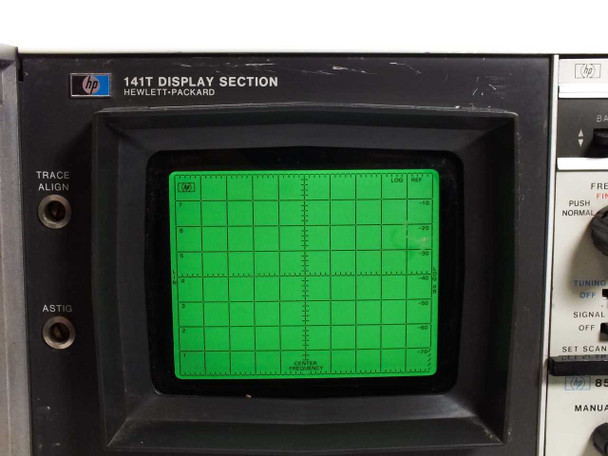
\includegraphics[width=0.62\textwidth]{Figures/Methodology/HP-Display-Section}
		\caption{HP141T \acrshort{crt} display section.}
		\label{fig:display-section}
	\end{figure}
	
	Secondary objectives include digitizing the operations that were previously executed by physical knobs such as horizontal and vertical scaling of the waveform. This objective can be  as functions in a program that can be called to perform similar task. The choice of coding language and available development tools for the program that runs the display is a critical part of the \acrshort{ui} subsystem. 
	
	An alternative approach to handling data acquisition and display functions on the same board would be to use a single-board computer for the display. Spectrum data can be retrieved from memory and displayed to the user in a Python, C/C++ or Java program. Knobs can be replaced by programmatic buttons with functions that users can access by touching the screen. This can allow other features such as averaging and displaying maxima and minima to be easily accessible to the user. For this project, \acrshort{ui} must enable users to select between different display modes, including the \acrshort{phm}, \acrshort{avm} and \acrshort{rwm}. The \acrshort{ui} must enable users to switch between these modes seamlessly and allow for back them to return to previous screens using a back button in the program.
	
	Overall, the project aims to adhere to Nielsen's heuristic design principles which includes:
	\begin{enumerate}
		\item
		Match between the system and the HP141T -  the program should use the language and current features of the HP141T that users are familiar with
		\item 
		User control and freedom - the \acrshort{ui} must support undo, redo and exit points
		\item 
		Aesthetics and minimalist design - the most relevant information that must be displayed is related to the frequency plot of the input signals as well as configurations and settings of the data acquisition and digital processing units that give context to the current display
		\item 
		Flexibility and efficiency of use - the \acrshort{ui} interface of the modernized HP141T must be optimized for difference experience levels through suitable shortcuts and frequent actions such as averaging and showing maxima and minima of the input signal.
		\item 
		Help and documentation - documentation of the modernized HP141T display must correspond to current documentations of the entire system and must be easy to read
		\item 
		Error prevention - the \acrshort{ui} must protect users from deleting stored traces and signal information
		\item 
		Visibility - a user must always know what is happening within the program and current state of their actions
		\item 
		Consistency and standards - the appearance of the \acrshort{ui} must follow the conventions of modern spectrum analyzer displays through consistent words, situations and actions.
		\item 
		Help user to recognize, diagnose and recover from errors such as closing windows with information about pulses or signal noise
		\item 
		Recognition rather than recall - minimize users' memory load by making program features that are related to the most accessed signal data easy to access
	\end{enumerate}
	
	\subsection{Equipment for Debugging and Testing}
	
	The following section gives a review of the project requirement which necessitates the development of an HP141T display emulator of the three auxiliary outputs as shown in \ref{tab:hp141t-output-voltages}. Additionally, the section describes software-based simulation tools that can be used in the development for debugging and obtaining an idea about the expected behaviour individual hardware components and overall system.
	
	\subsubsection{Emulating HP141T Auxiliary Outputs}
	
	The sawtooth signal can be generated using a 555-timer circuit which produces a ramp voltage with adjustable frequency to mimic the adjustable scan time, and a fixed peak-to-peak voltage of $\SI{10}{\volt}$ with no \acrshort{dc} offset. This is to ensure that the horizontal sawtooth output range between $-\SI{5}{\volt}$ and $+\SI{5}{\volt}$ is maintained. 
	
	To emulate the vertical output which swings between $\SI{0}{\volt}$ and $-\SI{0.8}{\volt}$, a simple voltage biasing circuit can be built with appropriate resistor values and input voltage. To control this level, a potentiometer can be used to manually adjust the voltage level within that range. Similarly, the pen-lift output can be produced using a biasing circuit with a potentiometer that allows the voltage to swing between $\SI{0}{\volt}$ and $\SI{14}{\volt}$. 
	
	Lastly, the HP141T display emulator circuit needs to interface with the signal conditioning circuit that prepares the signal voltages to match the operating range of the \acrshort{adc}. Therefore, to avoid the development of multiple circuits, the output cables of the display emulator must be the same as the output cables that take the auxiliary outputs from the HP141T to the signal conditioning circuit.
	
	\subsubsection{Software-Based Simulation Tools}
	
	To optimize the selection and configuration of the data acquisition subsystem, \acrshort{adc}s can be simulated in MATLAB using Simulink to understand the behaviour of the sawtooth input from the HP141T or emulating hardware. Additionally, Simulink provides visualizations of the spectrum of the \acrshort{adc} output which can be used to determine the expected values from sampling signals. Simulink also allows users to add impairments to the \acrshort{adc} for introducing a layer of non-linearity that may be seen for signals with frequencies that are close the edges of the \acrshort{rbw} or intermediate frequency. 
	
	Electronic circuits, such as the signal conditioning circuits with op-amps and level-shifters, can be simulated using LTSpice to predict the expected behaviour. Output values from LTSpice simulations can be used to simulate the behaviour of the system using Simulink with MATLAB.
			
	\section{System Design}
	
	Design decisions in formulating the specifications were informed by the requirement review in the previous section. This section aims to give a full description of the system and the interfaces between the different subsystems. The section begins with a visual representation of the system using a block diagram. Following the visual representation of the design, the section includes specifications and concludes with acceptance and integration tests. 
	
	\subsection{Overview System Block Diagram}
	
	The system block diagram shown in Figure \ref{fig:overall-system-block-diagram} below is a graphical overview of the different stages that an RF signal goes through before the amplitude vs frequency graph is displayed. The modernized HP141T maintains the basic analog signal processing functionality performed by the HP8555A \acrshort{rf} section and the HP8552B \acrshort{if} sections. The scope of the proposed design does not involve any changes to the signal processing components of the plug-in sections. However, the Signal Conditioning Subsystem (\acrshort{scs}) prepares the three auxiliary outputs from the HP552B \acrshort{if} section for the Data Acquisition Subsystem (\acrshort{das}) which requires input voltages in the range between $\SI{0}{\volt}$ and $\SI{3.3}{\volt}$. 	
	
	\begin{figure}[ht!]
	 	\centering
	 	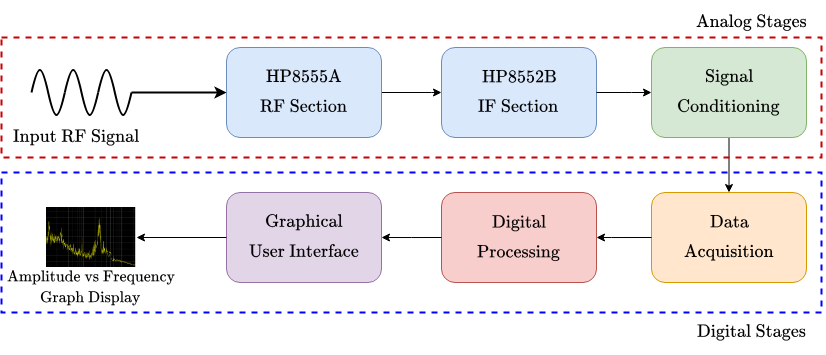
\includegraphics[width=0.80\textwidth]{Figures/Methodology/overall-system-diagram}
	 	\caption{Overview system block diagram for the modernized HP141T which employs the HP8555A and HP8552B plug-in sections.}
	 	\label{fig:overall-system-block-diagram}
	 \end{figure}
	\acrshort{adc}s in the \acrshort{das} play a primary role in digitizing the HP141T system by converting the conditioned analog signals into digital values which can be processed in the Digital Processing Subsystem (\acrshort{dps}) which enables manipulation of the digital values. This is particularly necessary for averaging and executing other arithmetic operations in order to satisfy the needs of the user. The Graphical User Interface Subsystem (\acrshort{guis}) manages the display and user preferences for displaying the amplitude vs frequency information of the input \acrshort{rf} signal.
		
	Overall, the can be modularized into five primary subsystems, including:
	\begin{enumerate}
		\item 
		HP141T Subsystem
		\item 
		Signal Conditioning (\acrshort{scs})
		\item 
		Data Acquisition (\acrshort{das})
		\item 
		Digital Processing (\acrshort{dps})
		\item 
		Graphical User Inferface (\acrshort{guis})
	\end{enumerate}
	
	Although this project does not involve the redesign of the HP141T subsystem, an HP141T Emulator design is proposed for simulating the outputs of the \acrshort{if} plug-in section. In particular, the emulator produces signals that are similar to the horizontal, vertical and pen lift outputs of the HP8552B plug-in. This implies that the emulator can be considered as a secondary subsystem that can substitute the HP141T subsystem during calibration of the digital section of the proposed design, as illustrated in figure \ref{fig:emulated-system-diagram}. Furthermore, the diagram illustrates that the emulator does not have high frequency input signals like the HP8555A \acrshort{rf} section plug-in. Instead, oscillators and function generator chips are proposed for producing outputs that approximate the auxiliary outputs, as shown in table \ref{tab:hp8552b-output-vals}.
	
	\begin{figure}[ht!]
		\centering
		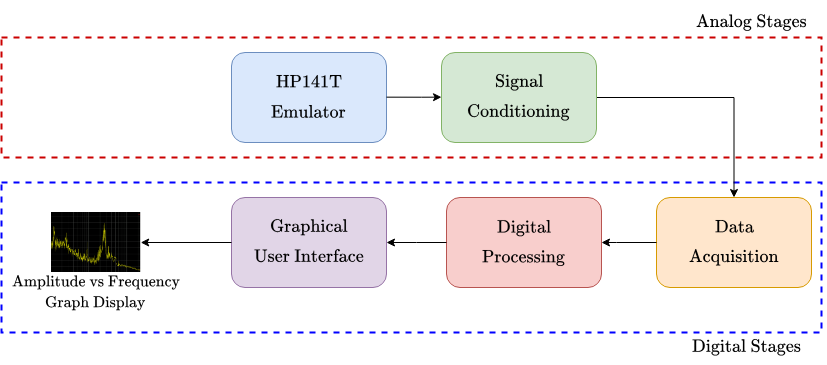
\includegraphics[width=0.80\textwidth]{Figures/Methodology/emulated-system-diagram}
		\caption{Calibration system diagram where the HP141T Emulator is used to configure the primary subsystems such as the \acrshort{scs}, \acrshort{das}, etc.}
		\label{fig:emulated-system-diagram}
	\end{figure}

	All analog stages are executed in \acrshort{pcb}s, and the digital stages are performed by a microcontroller and single-board computer. The following sections detail the specifications of the system modularization and components.

	\subsection{System Modularization}
	
	The system block diagram is expanded as illustrated in figure \ref{fig:system-block-diagram} where the primary components of each of the subsystems are shown. In the diagram, arrows with a solid line illustrate interfaces between subsystems, while arrows with dotted lines describes the flow of analog or digital signals within each subsystem.  
	\begin{figure}[ht!]
		\centering
		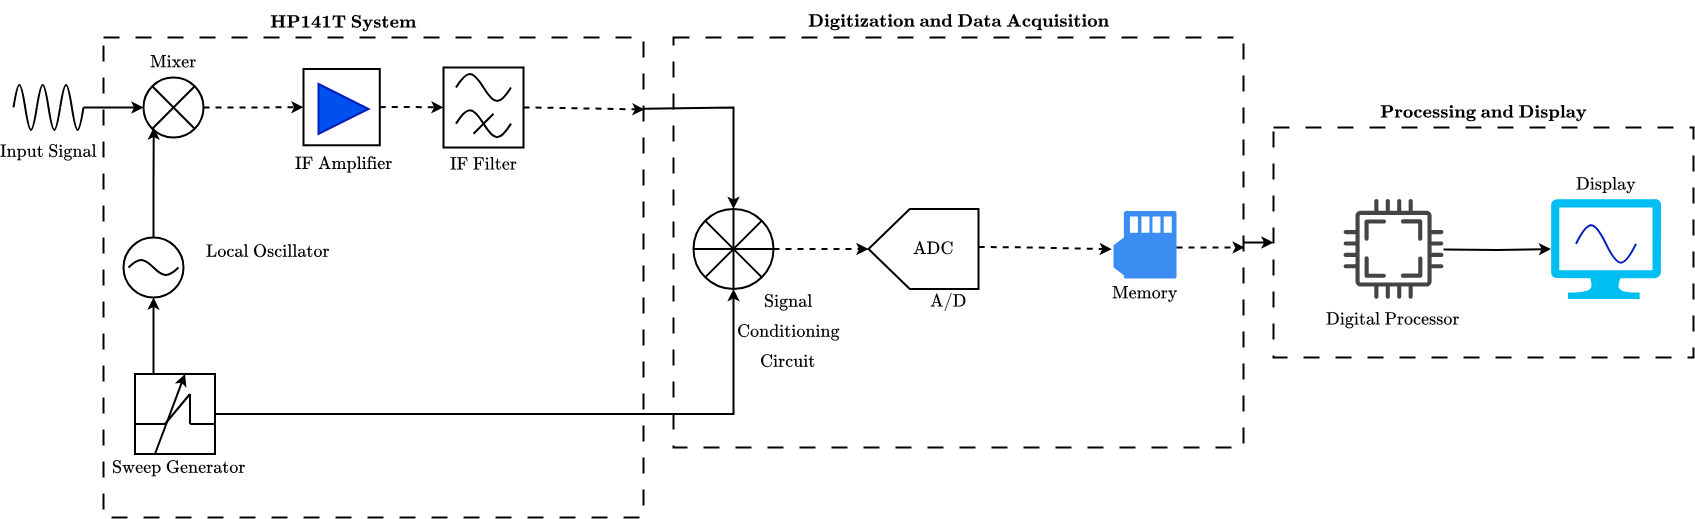
\includegraphics[width=0.90\textwidth]{Figures/Methodology/system-block-diagram}
		\caption{Expansion of the overall system diagram showing the primary components and functions in each subsystem.}
		\label{fig:system-block-diagram}
	\end{figure}
	\clearpage
	\begin{table}[ht!]
		\centering
		\label{tab:subsystem-components}
		\begin{tabular}{|m{18em}|m{15em}|m{8em}|}
			\hline
			\cellcolor{cyan!25}\textbf{Subsystem}	& \cellcolor{cyan!25}\textbf{Component}	& \cellcolor{cyan!25}\textbf{Signal Type}\\
			\hline
			\multirow{2}{*}{\textbf{HP141T Subsystem}}	& HP8555A	& Analog\\
			\cline{2-3}
														& HP8552B	& Analog\\
			\hline
			\multirow{3}{*}{\textbf{HP141T Emulator}}	& Vertical Output Simulator	& Analog\\
			\cline{2-3}
														& Horizontal Output Simulator & Analog\\
			\cline{2-3}
														& Pen Lift Output Simulator	& Analog\\
			\hline
			\multirow{3}{*}{\textbf{\acrlong{scs}}}	& Op-amp based vertical output conditioning circuit													& Analog\\
			\cline{2-3}
														& Op-amp based horizontal output conditioning circuit		& Analog\\
			\cline{2-3}
														& Op-amp based pen-lift output conditioning circuit 	& Analog\\
			\hline
			\multirow{3}{*}{\textbf{\acrlong{das}}}	& \acrshort{adc} & Analog/Digital\\
			\cline{2-3}
														& \acrshort{mcu} & Digital\\
			\cline{2-3}
														& Storage Device & Digital\\
			\hline
			\multirow{2}{*}{\textbf{\acrlong{dps}}}	& \acrshort{mcu} & Digital\\
			\cline{2-3}
														& \acrshort{sbc} & Digital\\
			\hline
			\multirow{3}{*}{\textbf{\acrlong{guis}}}	& \acrshort{sbc} & Digital\\
			\cline{2-3}
														& LCD Touch Screen & Digital/Analog\\
			\cline{2-3}
														& Software library & Digital \\
			\hline
		\end{tabular}
		\caption{Showing components in each subsystem and the type of signals that are processed by each unit.}
	\end{table}

	Figure \ref{fig:system-block-diagram} is accompanied by table \ref{tab:subsystem-components} showing subsystem components in more detail. The table also details the components of the HP141T Emulator subsystem. Signal types are noted in table \ref{tab:subsystem-components} because a significant part of the system behaviour can be attributed to the interchange between continuous or discrete values. 
	
	\subsubsection{HP141T Subsystem Specifications}
	
	Table \ref{tab:hp8552b-output-vals} shows the expected outputs collected from the technical manual of the plug-in which also details the expected frequency range. 
	\begin{table}[ht!]
		\centering
		\label{tab:hp8552b-output-vals}
		\begin{tabular}{|c|c|c|c|}
			\hline
			\cellcolor{cyan!25}\textbf{Output}	& \cellcolor{cyan!25}\textbf{Symbol}& \cellcolor{cyan!25}\textbf{Voltage Range}	& \cellcolor{cyan!25}\textbf{Bandwidth} \\
			\hline
			Horizontal & $\texttt{V}_\texttt{x}$	& $-\SI{5.0}{\volt}$ to $\SI{+5.0}{\volt}$	& $\SI{0.005}{\hertz}$ to $\SI{500}{\hertz}$\\
			\hline
			Vertical & $\texttt{V}_\texttt{y}$	& $-\SI{0.8}{\volt}$ to $\SI{0}{\volt}$	& $\SI{10}{\hertz}$ to $\SI{300}{\kilo\hertz}$\\
			\hline
			Pen Lift & $\texttt{V}_\texttt{z}$  & $\SI{0}{\volt}$ to $\SI{14}{\volt}$  & $\SI{0}{\hertz}$\\
			\hline
		\end{tabular}
		\caption{Characteristic values of the HP8552B \acrshort{if} plug-in section's analog output signals \cite{hp8552b}.}
	\end{table}

	Table \ref{tab:hp8552b-amplitude-specs} shows the amplitude specifications of the HP8552B plug-in section. 
	
	\begin{table}[ht!]
		\centering
		\label{tab:hp8552b-amplitude-specs}
		\begin{tabular}{|m{8em}|m{10em}|m{8em}|m{8em}|}
			\hline
			\cellcolor{cyan!25}\textbf{Operation Mode}	& \cellcolor{cyan!25}\textbf{Amplitude Calibration Range} & \cellcolor{cyan!25}\textbf{Amplitude per Division} ($\si{\decibel}$/div)	& \cellcolor{cyan!25}\textbf{Display Range} ($\si{\decibel}$)\\
			\hline
			Logarithmic & $-\SI{130}{\decibel}\text{m}$	to $+\SI{10}{\decibel}\text{m}$ & 10 & 70	\\
			\hline
			Linear & $-\SI{23}{\decibel\volt}$	to $+\SI{117}{\decibel\volt}$ 	& 10 & 70\\
			\hline
		\end{tabular}
		\caption{Amplitude specifications of HP8552B plug-in section \cite{hp8552b}.}
	\end{table}

	The HP8552B has four operational scan modes as shown in table \ref{tab:scan-specifications}. The table also shows the scan time specifications of the HP8552B. 
	
	\begin{table}[ht!]
		\centering
		\label{tab:scan-specifications}
		\begin{tabular}{|c|c|}
			\hline
			\cellcolor{cyan!25}\textbf{Scan Characteristic}	& \cellcolor{cyan!25}\textbf{Description} \\
			\hline
			Scan Time	& 16 scan rates from $\SI{0.1}{\milli\second}/\text{div}$ to $\SI{10}{\second}/\text{div}$ in a 1, 2, 5 sequence\\
			\hline
			\multirow{2}{*}{Scan Time Accuracy} & $\pm10\%$ for scan rates from $\SI{0.1}{\milli\second}/\text{div}$ to $\SI{20}{\milli\second}/\text{div}$\\
			\cline{2-2}
												& $\pm20\%$ for scan rates from $\SI{50}{\milli\second}/\text{div}$ to $\SI{10}{\second}/\text{div}$\\
			\hline
			\multirow{4}{*}{Scan Mode}	& \textit{Internal mode} for repetitive scanning by internally generated ramp	\\
			\cline{2-2}
										& \textit{Single mode} actuated by panel push button\\
			\cline{2-2}
										& \textit{External mode} determined by a $0$ to $+\SI{8}{\volt}$ external signal\\
			\cline{2-2}
										& \textit{Manual mode} controls the scan by the position of the manual knob\\
			\hline
			\multirow{4}{*}{Scan Trigger}	& \textit{Auto trigger} runs the scan freely\\
			\cline{2-2}
											&  \textit{Line trigger} synchronizes the scan with the power line frequency\\
			\cline{2-2}
											& \textit{External trigger} synchronizes the scan with an external signal ($\SI{20}{\volt}$ max) \\
			\cline{2-2}
											& \textit{Video trigger} synchronizes the scan to an envelope of the \acrshort{rf} input signal\\ 
			\hline
		\end{tabular}
		\caption{Scan time and scan mode specifications of the HP8552B plug-in \cite{hp8552b}.}
	\end{table}
		
	\subsubsection{HP141T Emulator Subsystem Design}
	
	The outputs of the HP141T emulator must be the same as three outputs of the HP8552B \acrshort{if} plug-in section as described in table \ref{tab:hp8552b-output-vals} above. The frequency range of the $\SI{-0.8}{\volt}-\SI{0}{\volt}$ vertical output, $\texttt{V}_\texttt{y}$, is limited to the bandwidth of the video filter in the \acrshort{if} section, i.e. $\SI{10}{\hertz}$ to $\SI{300}{\kilo\hertz}$ \cite{hp8552b}. The front panel check procedure in the technical manual of the HP8552B \acrshort{if} section sets a frequency range of up to $\SI{10}{\kilo\hertz}$ in the video filter, corresponding to a $\SI{30}{\mega\hertz}$ fundamental signal at the input of the \acrshort{rf} section plug-in \cite{HP8555A}.  
	
	\begin{figure}[h!]
		\centering
		\begin{subfigure}{.5\textwidth}
			\centering
			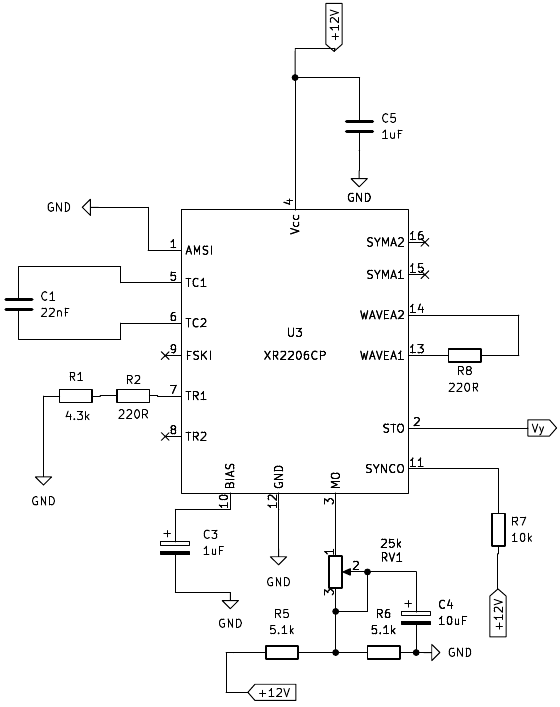
\includegraphics[width=.8\linewidth]{Figures/Methodology/hp8552b-vertical-output-emulator-3}
			\caption{Vertical output emulator circuit.}
			\label{fig:vertical-output-emulator-ct-a}
		\end{subfigure}%
		\begin{subfigure}{.5\textwidth}
			\centering
			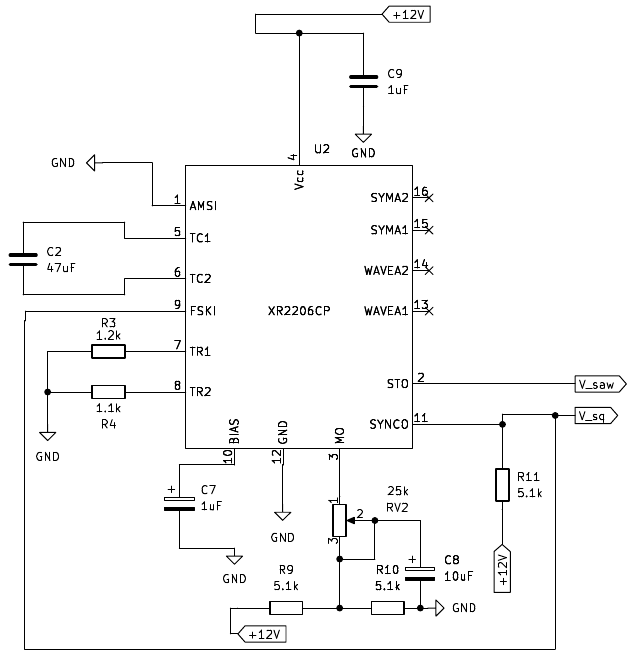
\includegraphics[width=.8\linewidth]{Figures/Methodology/hp8552b-horizontal-output-emulator-3}
			\caption{Horizontal output emulator circuit.}
			\label{fig:horizontal-output-emulator-ct-a}
		\end{subfigure}
		\caption{Emulator circuits for vertical and horizontal outputs of the HP8552B \acrshort{if} section.}
		\label{fig:hp8552B-vh-emulator}
	\end{figure}
	
	The XR2206 functional generator chip was selected for simulating the vertical and horizontal outputs, $\texttt{V}_\texttt{y}$ and $\texttt{V}_\texttt{x}$, respectively. For $\texttt{V}_\texttt{y}$, the circuit components were selected to simulate the video filter during the configuration procedure described in the chip's datasheet with a calibration frequency of $\SI{30}{\mega\hertz}$. The frequency was set to $\SI{10}{\kilo\hertz}$ using an capacitors and resistors. The full vertical output simulator circuit is illustrated in figure \ref{fig:vertical-output-emulator-ct-a}, adopted from the recommended configuration. 
		
	The required frequency is produced by an internal voltage-controlled oscillator that is set by a timing resistor at pin 7 and 8. Pin descriptions and the values of the capacitors and resistors that are connected to them are recorded in table \ref{tab:voec-pin-description} and \ref{tab:vertical-output-emulator-ct-specifications}.
	
%	\begin{table}[ht!]
%		\caption{Pin connection description for the XR2206-based vertical output simulation circuit.}
%		\label{tab:voec-pin-description}
%		\centering
%		\begin{tabular}{|m{3em}|c|c|m{10em}|m{18em}|}
%			\hline
%			\cellcolor{cyan!25}\textbf{Pin No.} & \cellcolor{cyan!25}\textbf{Type}	& \cellcolor{cyan!25}\textbf{Symbol} & \cellcolor{cyan!25}\textbf{Connection(s)} & \cellcolor{cyan!25}\textbf{Description} \\
%			\hline
%			1	&	I	& AMSI 	&	GND  & A $\SI{0}{\volt}$ amplitude modulation signal input.\\
%			\hline
%			2	&   O	& STO	&	$\texttt{V}_\texttt{y}$ & Sinusoid wave output.\\
%			\hline
%			3	& 	O	& MO	&	C8, RV2, R17, R18		& Multiplier output for controlling the amplitude of $\texttt{V}_\texttt{y}$\\
%			\hline
%			4	& 	I	& $\text{V}_{\text{CC}}$ & C7 & $+\SI{12}{\volt}$ power supply with decoupling capacitor.\\
%			\hline
%			5	& 	I	& TC1	&	C5			 & Timing capacitor.\\
%			\hline
%			6	&	I	& TC2	& 	C5			 & Timing capacitor.\\
%			\hline
%			7	&	O	& TR1	&	R15, R16	 & Timing resistor.\\
%			\hline
%			8	&	X	& TR2	&	X			 & No connection.\\
%			\hline
%			9	&	X	& FSKI	&	X			 & No connection.\\  
%			\hline
%			10	&	O	& BIAS	&	C6			 & Internal voltage reference.\\
%			\hline
%			11	&	O	& SYNCO	&	R20			 & Open collector with a pull-up resistor to the power
%			supply.\\
%			\hline
%			12	& 		& GND	&	GND			 & Ground pin.\\
%			\hline
%			13	&	I	& WAVEA1	&	R19		 & First waveform-adjustment input.\\
%			\hline
%			14	&	I	& WAVEA2	&	R19		 & Second waveform-adjustment input.\\
%			\hline
%			15	&	X	& SYMA1		&	X		 & No connection for wave symmetry adjustment.\\
%			\hline
%			16	&	X	& SYMA2		&	X		 & No connection for wave symmetry adjustment.\\
%			\hline
%		\end{tabular}
%	\end{table}

		\begin{table}[ht!]
		\caption{Pin connection description for the XR2206-based vertical output simulation circuit.}
		\label{tab:voec-pin-description}
		\centering
		\begin{tabular}{|m{3em}|c|m{10em}|m{18em}|}
			\hline
			\cellcolor{cyan!25}\textbf{Pin No.} & \cellcolor{cyan!25}\textbf{Type}	& \cellcolor{cyan!25}\textbf{Symbol} & \cellcolor{cyan!25}\textbf{Description} \\
			\hline
			1	&	I	& AMSI 	& A $\SI{0}{\volt}$ amplitude modulation signal input.\\
			\hline
			2	&   O	& STO	&	Sinusoid wave output.\\
			\hline
			3	& 	O	& MO	&	Multiplier output for controlling the amplitude of $\texttt{V}_\texttt{y}$\\
			\hline
			4	& 	I	& $\text{V}_{\text{CC}}$ & $+\SI{12}{\volt}$ power supply with decoupling capacitor.\\
			\hline
			5	& 	I	& TC1	&	Timing capacitor.\\
			\hline
			6	&	I	& TC2	& 	Timing capacitor.\\
			\hline
			7	&	O	& TR1	&	Timing resistor.\\
			\hline
			8	&	X	& TR2	&	 No connection.\\
			\hline
			9	&	X	& FSKI	&	No connection.\\  
			\hline
			10	&	O	& BIAS	&	 Internal voltage reference.\\
			\hline
			11	&	O	& SYNCO	&	 Open collector with a pull-up resistor to the power
			supply.\\
			\hline
			12	& 		& GND		& Ground pin.\\
			\hline
			13	&	I	& WAVEA1	&	 First waveform-adjustment input.\\
			\hline
			14	&	I	& WAVEA2	&	Second waveform-adjustment input.\\
			\hline
			15	&	X	& SYMA1		&	 No connection for wave symmetry adjustment.\\
			\hline
			16	&	X	& SYMA2		&	 No connection for wave symmetry adjustment.\\
			\hline
		\end{tabular}
	\end{table}
	The amplitude of $\texttt{V}_\texttt{y}$ and $\texttt{V}_\texttt{x}$ is controlled by adjusting the variable resistors $\text{RV1}$ and $\text{RV2}$, respectively.	To generate a sinusoid with a constant peak-to-peak voltage and constant frequency for the vertical output, an external capacitance of $\text{C} = \text{C}_1$ is connected across pin 5 and 6, and a timing resistance $\text{R} = \text{R}_1 + \text{R}_2$ across pin 7, such that the operational frequency $\texttt{f}_\texttt{y}$ of the XR2206 is 
	\begin{align}\label{eqn:xr2206-sinewave-frequency}
		\text{f}_y	& = \frac{1}{\text{R}\text{C}} ~ [\si{\hertz}]
	\end{align}
	Similarly, the characteristics of the horizontal sawtooth output depend on the timing components at pin 5, 6, and 7, as illustrated in figure \ref{fig:horizontal-output-emulator-ct-a}. However, when operating as a sawtooth function generator as in the case of the horizontal output emulator circuit, the frequency $\texttt{f}_y$ is given by,
	\begin{align}\label{eqn:xr2206-sawtooth-frequency}
		\text{f}_x	& = \frac{2}{\text{C}(\text{R}_a + \text{R}_b)} ~ [\si{\hertz}]
	\end{align}
	where $\text{R}_a$ and $\text{R}_b$ correspond to the timing resistors connected to pin 7 and pin 8, and $\text{C}$ is the timing capacitor connected to pin 5 and pin 6, respectively. The duty cycle of the output sawtooth function is given by the parallel combination of $\text{R}_a$ and $\text{R}_b$, such that 
	\begin{align}\label{eqn:xr2206-duty-cycle}
		\text{Duty Cycle}	& = \frac{\text{R}_a}{\text{R}_a + \text{R}_b}
	\end{align}
	The duty cycle is associated with the rise time, $\text{T}_\text{rise}$, of the sawtooth function in the output of the emulator as the scan voltage $\texttt{V}_\texttt{y}$ increases from the $\SI{0}{\volt}$ to $\SI{3}{\volt}$. The design approximates the rise time and duty cycle of this output found in the manual of the HP8552B and illustrated in figure \ref{fig:hp8552b-sawtooth} \cite{hp8552b}. Using $\text{R}_a = \text{R}_3 = \SI{1.1}{\kilo\ohm}$ and $\text{R}_b = \text{R}_4 = \SI{1.2}{\kilo\ohm}$, the duty cycle is approximated to $52.2\%$ and the rise time to $\SI{54}{\milli\second}$ of the XR2206 sawtooth output. The time domain characteristics corresponding to a horizontal oscillation frequency of $\SI{18.52}{\second}$, given that the timing capacitance is $\SI{47}{\micro\farad}$. 
	\begin{table}[ht!]
		\caption{H141T emulator electrical specifications.}
		\label{tab:vertical-output-emulator-ct-specifications}
		\centering
		\begin{tabular}{|cm{10em}m{5em}m{5em}m{5em}m{8em}|}
			\hline
			\cellcolor{cyan!25}\textbf{Designation} & \cellcolor{cyan!25}\textbf{Parameter} &	\cellcolor{cyan!25}\textbf{Minimum} &  \cellcolor{cyan!25}\textbf{Maximum}	& \cellcolor{cyan!25}\textbf{Units} & \cellcolor{cyan!25}\textbf{Conditions}\\
			\hline
			\multicolumn{6}{c}{\textbf{General Characteristics}}\\
			\hline
			$\text{V}_{\text{IN}}$ & Split Supply Voltage  & $10$ & $26$ & $\si{\volt}$ & \\
			\hline
			$\text{I}_{\text{IN}}$ & Supply Current  & $12$ & $17$ & $\si{\milli\ampere}$ & \\
			\hline
			\multicolumn{6}{c}{\textbf{Output Voltage Characteristics}}\\
			\hline
			$\texttt{V}_\texttt{y}$	& Vertical Output	&	$0$	&	$3$ & $\si{\volt}$ & $\text{RV1} = \SI{25}{\kilo\ohm}$ \\
			\hline
			$\texttt{V}_\texttt{x}$	& Horizontal Output	&	$-4.75$	&	$4.76$ & $\si{\volt}$ & $\text{RV2} = \SI{15}{\kilo\ohm}$\\
			\hline
			$\texttt{V}_\texttt{p}$	& Pen Lift Output	&   $0$	& 	$12$ & $\si{\volt}$ & \\
			\hline
			\multicolumn{6}{c}{\textbf{Frequency and Time Domain Characteristics}}\\
			\hline
			$\text{f}_\texttt{y}$	& Vertical Output Oscillation Frequency	&	&	$10$ & $\si{\kilo\hertz}$ & $\text{R}_1 = \SI{4.3}{\kilo\ohm}$, $\text{R}_2 = \SI{220}{\ohm}$, $\text{C}_1 = \SI{22}{\micro\farad}$ \\
			\hline
			$\text{f}_\texttt{x}$	& Horizontal Output Frequency	& $17.24$ 	& $20$ & $\si{\hertz}$ & $\text{R}_3 = \SI{1.2}{\kilo\ohm}$, $\text{R}_4 = \SI{1.3}{\ohm}$, $\text{C}_2 = \SI{47}{\micro\farad}$\\
			\hline
			$\text{T}_\text{rise}$				& Horizontal Output Sawtooth Rise Time	& $50$	&	$58$ &	$\si{\milli\second}$	&	$\text{R}_3 = \SI{1.2}{\kilo\ohm}$, $\text{R}_4 = \SI{1.3}{\ohm}$, $\text{C}_2 = \SI{47}{\micro\farad}$\\
			\hline
		\end{tabular}
	\end{table}
	\begin{figure}[ht!]
		\centering
		
\includegraphics[width=0.34\textwidth]{Figures/Methodology/hp8552b-sawtooth}
		\caption{Illustration of the duty cycle and rise time of sawtooth function corresponding to the horizontal output, $\texttt{V}_\texttt{x}$, of the HP8552B.}
		\label{fig:hp8552b-sawtooth}
	\end{figure}
	
	Since the output voltage of the multiplier and wave shaper in the XR2206 is limited between $\SI{0}{\volt}$ to $\SI{3}{\volt}$, the circuit in figure \ref{fig:emulator-circuit-level-shift} is used to adjust the sawtooth output from the chip to rise from $-\SI{5}{\volt}$ to $+\SI{5}{\volt}$.
	
	\begin{figure}[ht!]
		\centering
		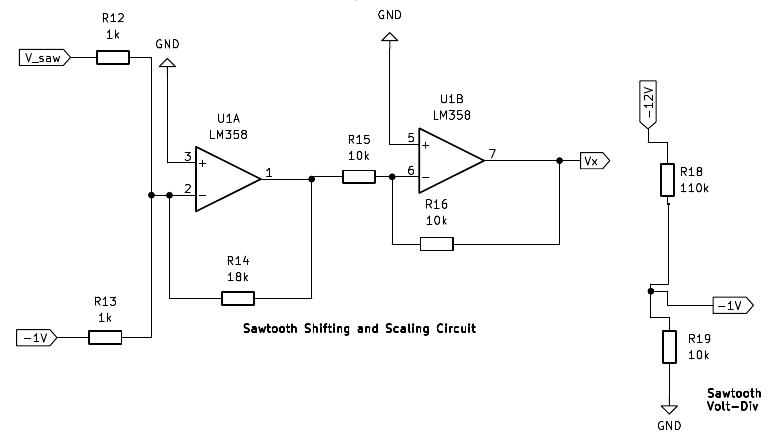
\includegraphics[width=0.50\textwidth]{Figures/Methodology/hp8552b-horizontal-output-level-shifter-3}
		\caption{XR2206 sawtooth output level shifter for achieving the appropriate voltage range.}
		\label{fig:emulator-circuit-level-shift}
	\end{figure}
	The circuit was simulated in LTSpice using the \texttt{PWL} command as shown in figure \ref{fig:sawtooth-sim-ltspice}, with the corresponding results of the simulation shown in the figure \ref{fig:sawtooth-sim-output}. The \texttt{PWL} command simulates a piecewise function from time t1 to time tn, $\text{n}\geq 2$. The simulation shows that the expected voltage range of the scan output lies between $-\SI{4.75}{\volt}$ and $\SI{4.76}{\volt}$ with a rapid rise time. This is due to the capacitors in the LM358 op-amp which introduce RC time constants during discharge. The steep rise time of the emulator is adjusted in software as specified in the following sections. 
	
	\begin{figure}[ht!]
		\centering
		
\includegraphics[width=0.55\linewidth]{Figures/Methodology/emulator-triangle-shift-ct-sim}
		\caption{Simulated level shift circuit.}
		\label{fig:sawtooth-sim-ltspice}
	\end{figure}

	\begin{figure}
		\centering
		
\includegraphics[width=0.7\linewidth]{Figures/Methodology/emulator-sawtooth-output}
		\caption{Showing simulated scan output of the emulator.}
		\label{fig:sawtooth-sim-output}
	\end{figure}

	
	\subsubsection{Signal Condition Subsystem Design}
	
	
	% ----------------------------------------------------
	\ifstandalone
	\bibliography{../Bibliography/References.bib}
	\printnoidxglossary[type=\acronymtype,nonumberlist]
	\fi
\end{document}
% ----------------------------------------------------